Zusätzlich zu Checkstyle haben wir das von Google entwickelte und empfohlene \glqq Android Lint\grqq~ genutzt. Dieses Tool ist speziell für Android optimiert und erzeugt im Gegensatz zu Checkstyle weniger Warnungen bezüglich syntaktischer Programmierrichtlinien, sondern vielmehr Empfehlungen zur Verbesserung der Performance, Usability, Accessibility und Korrektheit.

Dadurch verbessert sich einerseits die Wartbarkeit, denn durch das Befolgen der im Android-Umfeld üblichen Konventionen und die Verwendung von allgemein bekannten und anerkannten Entwurfsmustern, ist der Code zukünftigen Entwicklern leichter verständlich.

Im folgenden Abschnitt befindet sich wieder ein Report, der erstellt wurde, als wir begonnen haben, \glqq Android Lint\grqq~ einzusetzen. Dann wurden initial alle Warnungen und Empfehlungen abgearbeitet (Commit 1f4733747f7a98d89e7832937d94a9ddcbdc2bd5 \glqq fixes Android Lint errors and warnings\grqq). Die Warnungen und Empfehlungen werden direkt in der von uns verwendeten Entwicklungsumgebung Android Studio angezeigt, sodass diese anschließend während der Programmierung direkt umgesetzt werden konnten. Daher ist der zweite Report, der zum Abschluss des Projekts erstellt wurde, leer.

Nach den Berichten findet sich ein Screenshot, der markierte Android Lint-Warnungen anzeigt.


\includepdf[pages=1,offset=-0.8cm 0,scale=.8,pagecommand=\subsubsection{Initialer Android Lint Report}]{anhang/partials/lint-results-1.pdf}
\includepdf[pages=2-,offset=-0.8cm 0,scale=.8,pagecommand={}]{anhang/partials/lint-results-1.pdf}

\includepdf[pages=1,offset=-0.8cm 0,scale=.8,pagecommand=\subsubsection{Finaler Android Lint Report}]{anhang/partials/lint-results-2.pdf}

\subsubsection{Screenshot von Android Lint in Android Studio}

In diesem Screenshot ist ersichtlich, wie Android Lint anmerkt, statt \glqq paddingRight\grqq~ \glqq paddingEnd\grqq~ zu verwenden. Dies ist ein Beispiel für Verbesserungen der Accessibility für Android Apps. Weiterhin angemerkt wird, dass die beiden Konstruktionen aus jeweils einem \glqq LinearLayout\grqq~ und einem \glqq ImageView\grqq~ zu einem \glqq Compound Layout\grqq~ zusammengefasst werden können.

Durch die gelbe Hinterlegung in Android Studio, welche bereits beim Tippen des Quellcodes angezeigt wird, können Android Lint Warnungen kaum übersehen werden.

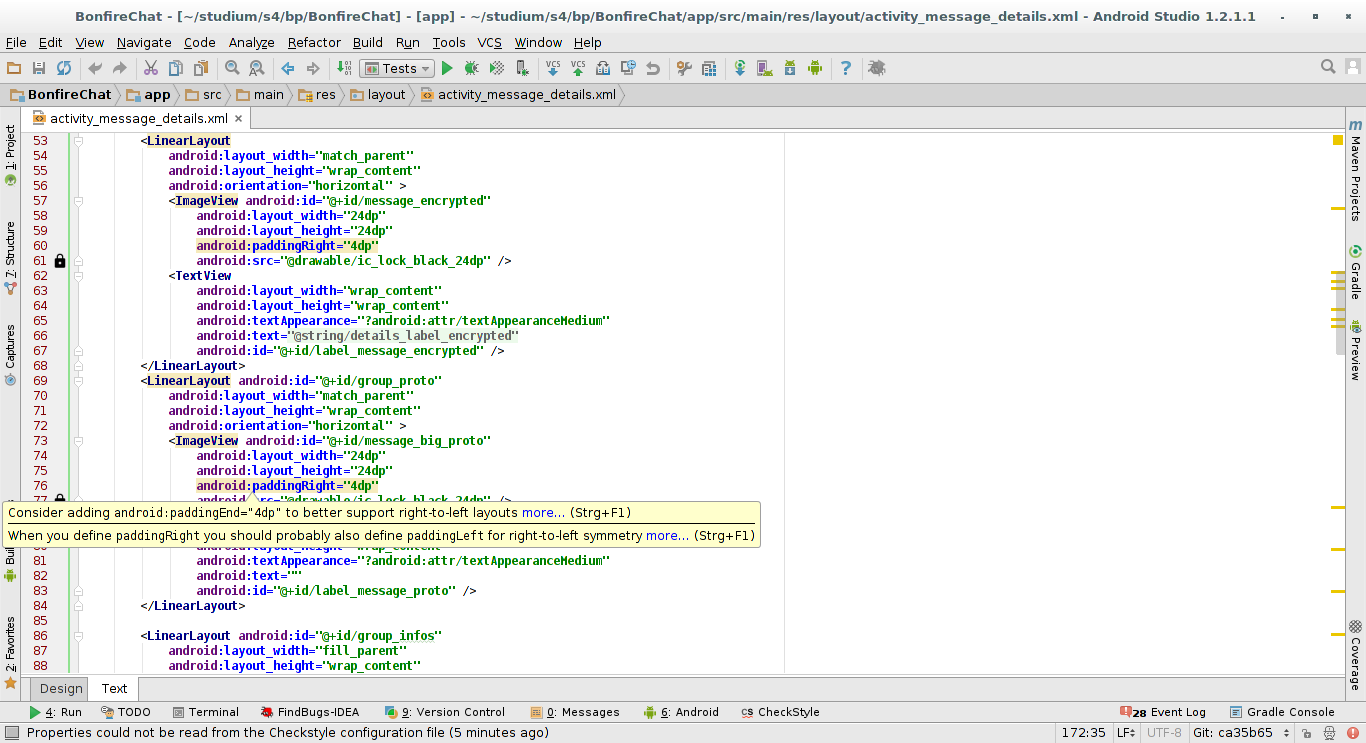
\includegraphics[width=17.5cm]{belege/lint/android-lint-screenshot.png}
